\documentclass[tikz]{standalone}
\usepackage{tikz}
\begin{document}
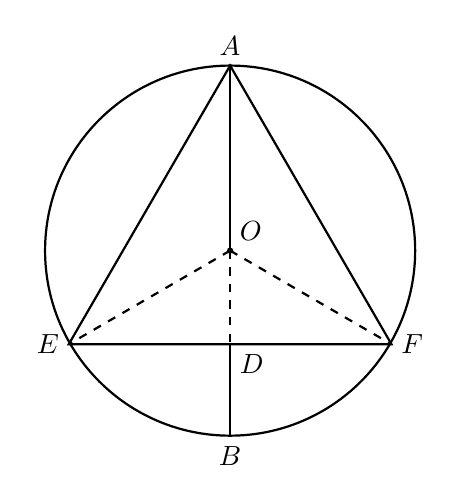
\begin{tikzpicture}[scale=1]
  % Coordinates
  \coordinate (O) at (0,0);
  \coordinate (A) at (0,2.35);
  \coordinate (B) at (0,-2.36);
  \coordinate (E) at (-2.05,-1.19);
  \coordinate (F) at (2.05,-1.19);
  \coordinate (D) at (0,-1.19);

  % Circumscribed circle
  \draw[thick] (O) circle (2.35);

  % Triangle AEF
  \draw[thick] (A) -- (E) -- (F) -- cycle;

  % Segment EF already drawn as triangle side; vertical line AB split at O and D
  \draw[thick] (A) -- (O);          % OA solid
  \draw[thick, dashed] (O) -- (D);  % DO dashed
  \draw[thick] (D) -- (B);          % BD solid

  % Dashed radii OE and OF
  \draw[thick, dashed] (O) -- (E);
  \draw[thick, dashed] (O) -- (F);

  % Center point
  \fill (O) circle (0.04);

  % Labels
  \node[above] at (A) {$A$};
  \node[below] at (B) {$B$};
  \node[left]  at (E) {$E$};
  \node[right] at (F) {$F$};
  \node[above right] at (O) {$O$};
  \node[below right] at (D) {$D$};
\end{tikzpicture}
\end{document}
